\documentclass[a4paper]{article}

\def\npart {IB}
\def\nterm {Lent}
\def\nyear {2016}
\def\nlecturer {R. E. Hunt}
\def\ncourse {Complex Methods}
\def\nlectures {MWF.9}
\def\nnotready {}

% Imports
\ifx \nextra \undefined
  \usepackage[pdftex,
    hidelinks,
    pdfauthor={Dexter Chua},
    pdfsubject={Cambridge Maths Notes: Part \npart\ - \ncourse},
    pdftitle={Part \npart\ - \ncourse},
  pdfkeywords={Cambridge Mathematics Maths Math \npart\ \nterm\ \nyear\ \ncourse}]{hyperref}
  \title{Part \npart\ - \ncourse}
\else
  \usepackage[pdftex,
    hidelinks,
    pdfauthor={Dexter Chua},
    pdfsubject={Cambridge Maths Notes: Part \npart\ - \ncourse\ (\nextra)},
    pdftitle={Part \npart\ - \ncourse\ (\nextra)},
  pdfkeywords={Cambridge Mathematics Maths Math \npart\ \nterm\ \nyear\ \ncourse\ \nextra}]{hyperref}

  \title{Part \npart\ - \ncourse \\ {\Large \nextra}}
\fi

\author{Lectured by \nlecturer \\\small Notes taken by Dexter Chua}
\date{\nterm\ \nyear}

\usepackage{alltt}
\usepackage{amsfonts}
\usepackage{amsmath}
\usepackage{amssymb}
\usepackage{amsthm}
\usepackage{booktabs}
\usepackage{caption}
\usepackage{enumitem}
\usepackage{fancyhdr}
\usepackage{graphicx}
\usepackage{mathtools}
\usepackage{microtype}
\usepackage{multirow}
\usepackage{pdflscape}
\usepackage{pgfplots}
\usepackage{siunitx}
\usepackage{tabularx}
\usepackage{tikz}
\usepackage{tkz-euclide}
\usepackage[normalem]{ulem}
\usepackage[all]{xy}

\pgfplotsset{compat=1.12}

\pagestyle{fancyplain}
\lhead{\emph{\nouppercase{\leftmark}}}
\ifx \nextra \undefined
  \rhead{
    \ifnum\thepage=1
    \else
      \npart\ \ncourse
    \fi}
\else
  \rhead{
    \ifnum\thepage=1
    \else
      \npart\ \ncourse\ (\nextra)
    \fi}
\fi
\usetikzlibrary{arrows}
\usetikzlibrary{decorations.markings}
\usetikzlibrary{decorations.pathmorphing}
\usetikzlibrary{positioning}
\usetikzlibrary{fadings}
\usetikzlibrary{intersections}
\usetikzlibrary{cd}

\newcommand*{\Cdot}{\raisebox{-0.25ex}{\scalebox{1.5}{$\cdot$}}}
\newcommand {\pd}[2][ ]{
  \ifx #1 { }
    \frac{\partial}{\partial #2}
  \else
    \frac{\partial^{#1}}{\partial #2^{#1}}
  \fi
}

% Theorems
\theoremstyle{definition}
\newtheorem*{aim}{Aim}
\newtheorem*{axiom}{Axiom}
\newtheorem*{claim}{Claim}
\newtheorem*{cor}{Corollary}
\newtheorem*{defi}{Definition}
\newtheorem*{eg}{Example}
\newtheorem*{fact}{Fact}
\newtheorem*{law}{Law}
\newtheorem*{lemma}{Lemma}
\newtheorem*{notation}{Notation}
\newtheorem*{prop}{Proposition}
\newtheorem*{thm}{Theorem}

\renewcommand{\labelitemi}{--}
\renewcommand{\labelitemii}{$\circ$}
\renewcommand{\labelenumi}{(\roman{*})}

\let\stdsection\section
\renewcommand\section{\newpage\stdsection}

% Strike through
\def\st{\bgroup \ULdepth=-.55ex \ULset}

% Maths symbols
\newcommand{\bra}{\langle}
\newcommand{\ket}{\rangle}

\newcommand{\N}{\mathbb{N}}
\newcommand{\Z}{\mathbb{Z}}
\newcommand{\Q}{\mathbb{Q}}
\renewcommand{\H}{\mathbb{H}}
\newcommand{\R}{\mathbb{R}}
\newcommand{\C}{\mathbb{C}}
\newcommand{\Prob}{\mathbb{P}}
\renewcommand{\P}{\mathbb{P}}
\newcommand{\E}{\mathbb{E}}
\newcommand{\F}{\mathbb{F}}
\newcommand{\cU}{\mathcal{U}}
\newcommand{\RP}{\mathbb{RP}}
\newcommand{\CP}{\mathbb{CP}}

\newcommand{\ph}{\,\cdot\,}

\DeclareMathOperator{\sech}{sech}
\DeclareMathOperator{\cosech}{cosech}
\DeclareMathOperator{\cosec}{cosec}

\DeclareMathOperator{\covol}{covol}
\DeclareMathOperator{\vol}{vol}

\let\Im\relax
\let\Re\relax
\DeclareMathOperator{\Im}{Im}
\DeclareMathOperator{\Re}{Re}
\DeclareMathOperator{\im}{im}
\DeclareMathOperator{\image}{image}
\DeclareMathOperator{\Ann}{Ann}

\DeclareMathOperator*{\res}{res}
\DeclareMathOperator{\Res}{Res}
\DeclareMathOperator{\Ind}{Ind}

\DeclareMathOperator{\tr}{tr}
\DeclareMathOperator{\diag}{diag}
\DeclareMathOperator{\rank}{rank}
\DeclareMathOperator{\card}{card}
\DeclareMathOperator{\spn}{span}
\DeclareMathOperator{\adj}{adj}

\DeclareMathOperator{\erf}{erf}
\DeclareMathOperator{\erfc}{erfc}

\DeclareMathOperator{\ord}{ord}
\DeclareMathOperator{\Sym}{Sym}

\DeclareMathOperator{\sgn}{sgn}
\DeclareMathOperator{\orb}{orb}
\DeclareMathOperator{\stab}{stab}
\DeclareMathOperator{\ccl}{ccl}

\DeclareMathOperator{\lcm}{lcm}
\DeclareMathOperator{\hcf}{hcf}

\DeclareMathOperator{\Int}{Int}
\DeclareMathOperator{\id}{id}

\DeclareMathOperator{\betaD}{beta}
\DeclareMathOperator{\gammaD}{gamma}
\DeclareMathOperator{\Poisson}{Poisson}
\DeclareMathOperator{\binomial}{binomial}
\DeclareMathOperator{\multinomial}{multinomial}
\DeclareMathOperator{\Bernoulli}{Bernoulli}
\DeclareMathOperator{\like}{like}

\DeclareMathOperator{\var}{var}
\DeclareMathOperator{\cov}{cov}
\DeclareMathOperator{\bias}{bias}
\DeclareMathOperator{\mse}{mse}
\DeclareMathOperator{\corr}{corr}

\DeclareMathOperator{\otp}{otp}
\DeclareMathOperator{\dom}{dom}

\DeclareMathOperator{\Root}{Root}
\DeclareMathOperator{\supp}{supp}
\DeclareMathOperator{\rel}{rel}
\DeclareMathOperator{\Hom}{Hom}
\DeclareMathOperator{\Aut}{Aut}
\DeclareMathOperator{\Gal}{Gal}
\DeclareMathOperator{\Mat}{Mat}
\DeclareMathOperator{\End}{End}
\DeclareMathOperator{\Char}{char}
\DeclareMathOperator{\ev}{ev}
\DeclareMathOperator{\St}{St}
\DeclareMathOperator{\Lk}{Lk}
\DeclareMathOperator{\disc}{disc}
\DeclareMathOperator{\Isom}{Isom}
\DeclareMathOperator{\length}{length}
\DeclareMathOperator{\energy}{energy}
\DeclareMathOperator{\area}{area}
\DeclareMathOperator{\Syl}{Syl}
\DeclareMathOperator{\cl}{cl}
\DeclareMathOperator{\fix}{fix}

\newcommand{\GL}{\mathrm{GL}}
\newcommand{\SL}{\mathrm{SL}}
\newcommand{\PGL}{\mathrm{PGL}}
\newcommand{\PSL}{\mathrm{PSL}}
\newcommand{\PSU}{\mathrm{PSU}}
\newcommand{\Or}{\mathrm{O}}
\newcommand{\SO}{\mathrm{SO}}
\newcommand{\U}{\mathrm{U}}
\newcommand{\SU}{\mathrm{SU}}

\renewcommand{\d}{\mathrm{d}}
\newcommand{\D}{\mathrm{D}}

\tikzset{->/.style = {decoration={markings,
                                  mark=at position 1 with {\arrow[scale=2]{latex'}}},
                      postaction={decorate}}}
\tikzset{<-/.style = {decoration={markings,
                                  mark=at position 0 with {\arrowreversed[scale=2]{latex'}}},
                      postaction={decorate}}}
\tikzset{<->/.style = {decoration={markings,
                                   mark=at position 0 with {\arrowreversed[scale=2]{latex'}},
                                   mark=at position 1 with {\arrow[scale=2]{latex'}}},
                       postaction={decorate}}}
\tikzset{->-/.style = {decoration={markings,
                                   mark=at position #1 with {\arrow[scale=2]{latex'}}},
                       postaction={decorate}}}
\tikzset{-<-/.style = {decoration={markings,
                                   mark=at position #1 with {\arrowreversed[scale=2]{latex'}}},
                       postaction={decorate}}}

\tikzset{circ/.style = {fill, circle, inner sep = 0, minimum size = 3}}
\tikzset{mstate/.style={circle, draw, blue, text=black, minimum width=0.7cm}}

\definecolor{mblue}{rgb}{0.2, 0.3, 0.8}
\definecolor{morange}{rgb}{1, 0.5, 0}
\definecolor{mgreen}{rgb}{0.1, 0.4, 0.2}
\definecolor{mred}{rgb}{0.5, 0, 0}

\def\drawcirculararc(#1,#2)(#3,#4)(#5,#6){%
    \pgfmathsetmacro\cA{(#1*#1+#2*#2-#3*#3-#4*#4)/2}%
    \pgfmathsetmacro\cB{(#1*#1+#2*#2-#5*#5-#6*#6)/2}%
    \pgfmathsetmacro\cy{(\cB*(#1-#3)-\cA*(#1-#5))/%
                        ((#2-#6)*(#1-#3)-(#2-#4)*(#1-#5))}%
    \pgfmathsetmacro\cx{(\cA-\cy*(#2-#4))/(#1-#3)}%
    \pgfmathsetmacro\cr{sqrt((#1-\cx)*(#1-\cx)+(#2-\cy)*(#2-\cy))}%
    \pgfmathsetmacro\cA{atan2(#2-\cy,#1-\cx)}%
    \pgfmathsetmacro\cB{atan2(#6-\cy,#5-\cx)}%
    \pgfmathparse{\cB<\cA}%
    \ifnum\pgfmathresult=1
        \pgfmathsetmacro\cB{\cB+360}%
    \fi
    \draw (#1,#2) arc (\cA:\cB:\cr);%
}
\newcommand\getCoord[3]{\newdimen{#1}\newdimen{#2}\pgfextractx{#1}{\pgfpointanchor{#3}{center}}\pgfextracty{#2}{\pgfpointanchor{#3}{center}}}

\def\Xint#1{\mathchoice
   {\XXint\displaystyle\textstyle{#1}}%
   {\XXint\textstyle\scriptstyle{#1}}%
   {\XXint\scriptstyle\scriptscriptstyle{#1}}%
   {\XXint\scriptscriptstyle\scriptscriptstyle{#1}}%
   \!\int}
\def\XXint#1#2#3{{\setbox0=\hbox{$#1{#2#3}{\int}$}
     \vcenter{\hbox{$#2#3$}}\kern-.5\wd0}}
\def\ddashint{\Xint=}
\def\dashint{\Xint-}


\begin{document}
\maketitle
{\small
\noindent\textbf{Analytic functions}\\
Definition of an analytic function. Cauchy-Riemann equations. Analytic functions as conformal mappings; examples. Application to the solutions of Laplace's equation in various domains. Discussion of $\log z$ and $z^a$.\hspace*{\fill} [5]

\vspace{10pt}
\noindent\textbf{Contour integration and Cauchy's Theorem}\\
{[}\emph{Proofs of theorems in this section will not be examined in this course.}{]}\\
Contours, contour integrals. Cauchy's theorem and Cauchy's integral formula. Taylor and Laurent series. Zeros, poles and essential singularities.\hspace*{\fill} [3]

\vspace{10pt}
\noindent\textbf{Residue calculus}\\
Residue theorem, calculus of residues. Jordan's lemma. Evaluation of definite integrals by contour integration.\hspace*{\fill} [4]

\vspace{10pt}
\noindent\textbf{Fourier and Laplace transforms}\\
Laplace transform: definition and basic properties; inversion theorem (proof not required); convolution theorem. Examples of inversion of Fourier and Laplace transforms by contour integration. Applications to differential equations.\hspace*{\fill} [4]}

\tableofcontents

\setcounter{section}{-1}
\section{Introduction}
This is a methods course. By this, we mean we will not focus too much on proofs. We will at best just skim over the proofs. Instead, we focus on \emph{doing things}. We will not waste time proving things people have proved 300 years ago. If you like proofs, you can go to the IB Complex Analysis course, or look them up in relevant books.

\section{Analytic functions}
\subsection{The complex plane and the Riemann sphere}
We begin with a review of complex numbers. Any complex number $z \in \C$ can be written in the form $x + iy$, where $x = \Re z$, $y = \Im z$ are real numbers. We can also write it as $r e^{i\theta}$, where
\begin{defi}[Modulus and argument]
  The \emph{modulus} and \emph{argument} of a complex number $z = x + iy$ are given by
  \[
    r = |z| = \sqrt{x^2 + y^2}, \quad \theta = \arg z,
  \]
  where $x \tan \theta = y$.
\end{defi}
The argument is defined only up to multiples of $2\pi$. So we define the following:
\begin{defi}[Principal value of argument]
  The \emph{principal value} of the argument is the value of $\theta$ in the range $(-\pi, \pi]$.
\end{defi}
Note that the formula $\tan^{-1} \left(\frac{y}{x}\right)$ does not always give the right answer --- it is correct only if $x > 0$. If $x \leq 0$, then it might be out by $\pm \pi$ (eg. consider $z = 1 + i$ and $z = -1 - i$).

\begin{defi}[Open set]
  An \emph{open set} $\mathcal{D}$ is one which does not include its boundary. More technically, $\mathcal{D} \subseteq \C$ is open if for all $z_0 \in \mathcal{D}$, there is some $\delta > 0$ such that the disc $|z - z_0| < \delta$ is contained in $\mathcal{D}$.
\end{defi}

\begin{defi}[Neighbourhood]
  A \emph{neighbourhood} of a point $z \in \C$ is an open set containing $z$.
\end{defi}

\subsubsection*{The extended complex plane}
\begin{defi}[The extended complex plane]
  The \emph{extended complex plane} is $\C^* = \C \cup \{\infty\}$. We can reach the ``point at infinity'' by going off in any direction in the plane, and all are equivalent. In particular, there is no concept of $-\infty$. All infinities are the same. Operations with $\infty$ are done in the obvious way.
\end{defi}
Sometimes, we \emph{do} write down things like $-\infty$. This does not refer to a different point. Instead, this indicates a \emph{limiting process}. We mean we are approaching this infinity from the direction of the negative real axis. However, we still end up in the same place.

Conceptually, we can use the \emph{Riemann sphere}, which is a sphere resting on the complex plane with its ``South Pole'' $S$ at $z = 0$.
\begin{center}
  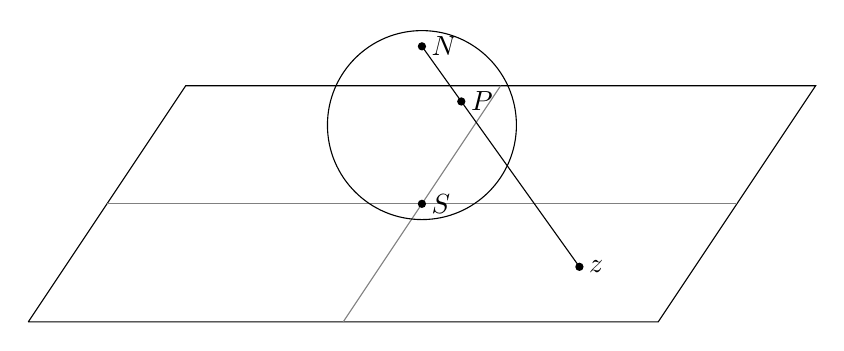
\begin{tikzpicture}
    \draw (0, 0) -- (8, 0) -- (10, 3) -- (2, 3) -- (0, 0);
    \draw [gray] (1, 1.5) -- (9, 1.5);
    \draw [gray] (4, 0) -- (6, 3);
    \draw (5, 2.5) circle [radius=1.2];

    \node [circ] at (5, 1.5) {};
    \node at (5, 1.5) [right] {$S$};

    \node [circ] at (5, 3.5) {};
    \node at (5, 3.5) [right] {$N$};

    \node [circ] at (5.5, 2.8) {};
    \node at (5.5, 2.8) [right] {$P$};

    \draw (5, 3.5) -- (7, 0.7) node [circ] {} node [right] {$z$};
  \end{tikzpicture}
\end{center}
 % improve
For any point $z \in \C$, drawing a line through the ``North Pole'' $N$ of the sphere to $z$, and noting where this intersects the sphere. This specifies an equivalent point $P$ on the sphere. Then $\infty$ is equivalent to the North Pole of the sphere itself. So the extended complex plane is mapped bijectively to the sphere.

To investigate properties of $\infty$, we use the substitution $\zeta = \frac{1}{z}$. A function $f(z)$ is said to have a particular property \emph{at $\infty$} if $f(\frac{1}{\zeta})$ has that same property at $\zeta = 0$. This vague notion will be made precise when we have specific examples to play with.

\subsection{Complex differentiation}
Recall the definition of differentiation for a real function $f(x)$:
\[
  f'(x) = \lim_{\delta x \to 0} \frac{f(x + \delta x) - f(x)}{\delta x}.
\]
It is implicit that the limit must be the same whichever direction we approach from. For example, consider $|x|$ at $x = 0$. If we approach from the right, ie. $\delta x \to 0^+$, then the limit is $+1$, whereas from the left, ie. $\delta x \to 0^-$, the limit is $-1$. Because these limits are different, we say that $|x|$ is not differentiable at the origin.

This is obvious and we already know that, but for complex differentiation, this issue is much more important, since there are many more directions. We now extend the definition of differentiation to complex number:
\begin{defi}[Complex differentiable function]
  A complex differentiable function $f: \C \to \C$ is \emph{differentiable} at $z$ if
  \[
    f'(z) = \lim_{\delta z \to 0} \frac{f(z + \delta z) - f(z)}{\delta z}
  \]
  exists (and is therefore independent of the direction of approach --- but now there are infinitely many possible directions).
\end{defi}

\begin{defi}[Analytic function]
  We say $f$ is \emph{analytic} at a point $z$ if there exists a neighbourhood of $z$ throughout which $f'$ exists. The terms \emph{regular} and \emph{holomorphic} are also used.
\end{defi}
In complex analysis, this sentence might be a few paragraphs long instead. Usually ``holomorphic'' is defined to mean the function has a Taylor series, but then we go on to prove that having a Taylor series is the same as being differentiable in a neighbourhood, ie. being holomorphic and analytic are the same.

\begin{defi}[Entire function]
  A complex function is \emph{entire} if it is analytic throughout $\C$.
\end{defi}

The property of analyticity is in fact a surprisingly strong one! For example, two consequences are:
\begin{enumerate}
  \item If a function is analytic, then it is differentiable infinitely many times. This is very \emph{very} false for real functions. There are real functions differentiable $N$ times, but no more (eg. by taking a non-differentiable function and integrating it $N$ times).
  \item A bounded entire function must be a constant.
\end{enumerate}
There are many more interesting properties, but these are sufficient to show us that complex differentiation is very different from real differentiation.
\subsubsection*{The Cauchy-Riemann equations}
We start by separating $f$ and $z$ into real and imaginary parts, ie.
\[
  f(z) = u(x, y) + iv(x, y),
\]
where $z = x + iy$ are $u, v$ are real functions.

We suppose that $f$ is differentiable at $z$. We may take $\delta z$ in any direction we like. First, we take it to be real, with $\delta z = \delta x$. Then
\begin{align*}
  f'(z) &= \lim_{\delta x \to 0} \frac{f(z + \delta x) - f(z)}{\delta x}\\
  &= \lim_{\delta x \to 0} \frac{u(x + \delta x, y) + iv(x + \delta x, y) - (u(x, y) + iv(x, y))}{\delta x}\\
  &= \frac{\partial u}{\partial x} + i \frac{\partial v}{\partial x}.
\end{align*}
What this says is something entirely obvious --- since we are allowed to take the limit in any direction, we can take it in the $x$ direction, and we get the corresponding partial derivative. This is a completely uninteresting point. Instead, let's do the really fascinating thing of taking the limit in the $y$ direction!

Let $\delta z = i \delta y$. Then we can compute
\begin{align*}
  f'(z) &= \lim_{\delta y \to 0} \frac{f(z + i\delta y) - f(z)}{i \delta y}\\
  &= \lim_{\delta y \to 0} \frac{u(x, y + \delta y) + iv(x, y + \delta y) - (u(x, y) + iv(x, y))}{i \delta y}\\
  &= \frac{\partial v}{\partial y} - i \frac{\partial u}{\partial y}.
\end{align*}
By the definition of differentiability, the two results for $f'(z)$ must agree! So we must have
\[
  \frac{\partial u}{\partial x} + i \frac{\partial v}{\partial x} = \frac{\partial v}{\partial y} - i \frac{\partial u}{\partial y}.
\]
Taking the real and imaginary components, we get
\begin{prop}[Cauchy-Riemann equations]
  If $f = u + iv$ is differentiable, then
  \[
    \frac{\partial u}{\partial x} = \frac{\partial v}{\partial y},\quad \frac{\partial u}{\partial y} = -\frac{\partial v}{\partial x}.
  \]
\end{prop}
Is the converse true? If these equations hold, does it follow that $f$ is differentiable? This is not always true. This holds only if $u$ and $v$ themselves are differentiable, which is a stronger condition that the partial derivatives exist, as you may have learnt from IB Analysis II. In particular, this holds if the partial derivatives $u_x, u_y, v_x, v_y$ are continuous (which implies differentiability).

\subsubsection*{Examples of analytic functions}
\begin{eg}\leavevmode
  \begin{enumerate}
    \item $f(z) = z$ is entire, ie. differentiable everywhere. Here $u = x, v = y$. Then the Cauchy-Riemann equations are satisfied everywhere, since
      \[
        \frac{\partial u}{\partial x} = \frac{\partial v}{\partial y} = 1,\quad \frac{\partial u}{\partial y} = -\frac{\partial v}{\partial x} = 0,
      \]
      and these are clearly continuous. Alternatively, we can prove this directly from the definition.
    \item $f(z) = e^z = e^x (\cos y + i \sin y)$ is entire since
      \[
        \frac{\partial u}{\partial x} = e^x \cos y = \frac{\partial v}{\partial y},\quad \frac{\partial u}{\partial y} = - e^x \sin y = -\frac{\partial v}{\partial x}.
      \]
      The derivative is
      \[
        f'(z) = \frac{\partial u}{\partial x} + i \frac{\partial v}{\partial x} = e^x \cos y + i e^x \sin y = e^z,
      \]
      as expected.
    \item $f(z) = z^n$ for $n \in \N$ is entire. This is less straightforward to check. Writing $z = r(\cos \theta + i \sin \theta)$, we obtain
      \[
        u = r^n \cos n\theta,\quad v = r^n \sin n\theta.
      \]
      We can check the Cauchy-Riemann equation using the chain rule, writing $r = \sqrt{x^2 = y^2}$ and $\tan \theta = \frac{y}{x}$. This takes quite a while, and it's not worth your time. But if you really do so, you will find the derivative to be $nz^{n - 1}$.
    \item Any rational function, ie. $f(z) = \frac{P(z)}{Q(z)}$ where $P, Q$ are polynomials, is analytic \emph{except} at points where $Q(z) = 0$ (where it is not even defined). For instance,
      \[
        f(z) = \frac{z}{z^2 + 1}
      \]
      is analytic except at $\pm i$.
    \item Many standard functions can be extended naturally to complex functions and obey the usual rules for their derivatives. For example,
      \begin{itemize}
        \item $\sin z = \frac{e^{iz} - e^{-iz}}{2i}$ is differentiable with derivative $\cos z = \frac{e^{iz} + e^{-iz}}{2}$. We can also write
          \begin{align*}
            \sin z &= \sin (x + iy) \\
            &= \sin x \cos iy + \cos x \sin iy \\
            &= \sin x \cosh y + i \cos x \sinh y.
          \end{align*}
        \item Similarly $\cos z, \sinh z, \cosh z$ etc. differentiate to what we expect them to differentiate to.
        \item $\log z = \log|z| + i \arg z$ has derivative $\frac{1}{z}$.
        \item The product rule, quotient rule and chain rule hold in exactly the same way, which allows us to prove (iii) and (iv) easily.
      \end{itemize}
  \end{enumerate}
\end{eg}

\subsubsection*{Examples of non-analytic functions}
\begin{eg}\leavevmode
  \begin{enumerate}
    \item Let $f(z) = \Re z$. This has $u = x, v = 0$. But
      \[
        \frac{\partial u}{\partial x} = 1\not= 0 = \frac{\partial v}{\partial y}.
      \]
      So $\Re z$ is nowhere analytic.
    \item Consider $f(z) = |z|$. This has $u = \sqrt{x^2 + y^2} = 0, v = 0$. This is thus nowhere analytic.
    \item The complex conjugate $f(z) = \bar z = z^* = x - iy$ has $u = x, v = -y$. So the Cauchy-Riemann equations don't hold. Hence this is nowhere analytic.

      We could have deduced (ii) from this --- if $|z|$ were analytic, then so would $|z|^2$, and hence $\bar{z} = \frac{|z|^2}{z}$ also has to be analytic.
    \item We have to be a bit more careful with $f(z) = |z|^2 = x^2 + y^2$. The Cauchy-Riemann equations are satisfied only at the origin. So $f$ is only differentiable at $z = 0$. However, it is not analytic since there is no neighbourhood of $0$ throughout which $f$ is differentiable.
  \end{enumerate}
\end{eg}

\subsection{Harmonic functions}
This is the last easy section of the course.

\begin{defi}[Harmonic conjugates]
  Functions $u, v$ satisfying the Cauchy-Riemann equations are called \emph{harmonic conjugates}.
\end{defi}

If we know one, then we can find the other up to a constant. For example, if $u(x, y) = x^2 - y^2$, then $v$ must satisfy
\[
  \frac{\partial v}{\partial y} = \frac{\partial u}{\partial x} = 2x.
\]
So we must have $v = 2xy + g(x)$ for some function $g(x)$. The other Cauchy-Riemann equation gives
\[
  -2y = \frac{\partial u}{\partial y} = -\frac{\partial v}{\partial x} = -2y - g'(x).
\]
This tells us $g'(x) = 0$. So $g$ must be a genuine constant, say $\alpha$. The corresponding analytic function whose real part is $u$ is therefore
\[
  f(z) = x^2 - y^2 + 2ixy + i\alpha = (x + iy)^2 + i \alpha = z^2 + i\alpha.
\]
Note that in an exam, if we were asked to find the analytic function $f$ with real part $u$ (where $u$ is given), then we \emph{must} express it in terms of $z$, and not $x$ and $y$, or else it is not clear this is indeed analytic.

On the other hand, if $f(z) = u + iv$ is analytic, then we can compute
\begin{align*}
  \frac{\partial^2 u}{\partial x^2} &= \frac{\partial }{\partial x}\left(\frac{\partial u}{\partial x}\right)\\
  &= \frac{\partial }{\partial x} \left(\frac{\partial v}{\partial y}\right)\\
  &= \frac{\partial }{\partial y}\left(\frac{\partial v}{\partial x}\right)\\
  &= \frac{\partial }{\partial y}\left(- \frac{\partial u}{\partial y}\right)\\
  &= -\frac{\partial^2 u}{\partial y^2}.
\end{align*}
So $u$ satisfies Laplace's equation in two dimensions, ie.
\[
  \nabla^2 u = \frac{\partial^2 u}{\partial x^2} + \frac{\partial^2 u}{\partial y^2} = 0.
\]
Similarly, so does $v$.
\begin{defi}[Harmonic function]
  A function satisfying Laplace's equation equation in an open set is said to be \emph{harmonic}.
\end{defi}

Thus we have shown the following:
\begin{prop}
  The real and imaginary parts of any analytic function are harmonic.
\end{prop}

\subsection{Multi-valued functions}
For $z = r^{i\theta}$, we define $\log z = \log r + i \theta$. There are infinitely many values of $\log z$, for every choice of $\theta$. For example,
\[
  \log i = \frac{\pi i}{2} \text{ or }\frac{5\pi i}{2}\text{ or } -\frac{3\pi i}{2}\text{ or }\cdots.
\]
This is fine, right? Functions can be multi-valued. Nothing's wrong.

Well, when we write down an expression, it'd better be well-defined. So we really should find some way to deal with this.

This section is really more subtle than it sounds like. It turns out it is non-trivial to deal with these multi-valued functions. We can't just, say, randomly require $\theta$ to be in, say, $\left(0, 2\pi\right]$, or else we will have some continuity problems, as we will later see.

\subsubsection*{Branch points}
Consider the three curves shown in the diagram.
\begin{center}
  \begin{tikzpicture}
    \draw [->] (-3, 0) -- (3, 0);
    \draw [->] (0, -3) -- (0, 3);
    \draw [->] (1, 1) arc (45:405:1.41) node [anchor = south west] {$C_3$};

    \draw [->] (3, 3) arc(0:360:1) node [right] {$C_1$};
    \draw [->] (-2, 0) arc(0:360:0.4) node [anchor = south west] {$C_2$};
  \end{tikzpicture}
\end{center}
In $C_1$, we could always choose $\theta$ to be always in the range $\left(0, \frac{\pi}{2}\right)$, and then $\log z$ would be continuous and single-valued going round $C_1$.

On $C_2$, we could choose $\theta \in \left(\frac{\pi}{2}, \frac{3\pi}{2}\right)$ and $\log z$ would again be continuous and single-valued.

However, this doesn't work for $C_3$. Since this encircles the origin, there is no such choice. Whatever we do, $\log z$ cannot be made continuous and single-valued around $C_3$. It must either ``jump'' somewhere, or the value has to increase by $2\pi i$ every time we go round the circle, ie. the function is multi-valued.

We now define what a branch point is. In this case, it is the origin, since that is where all our problems occur.
\begin{defi}[Branch point]
  A \emph{branch point} of a function is a point which is impossible to encircle with a curve on which the function is both continuous and single-valued. The function is said to have a \emph{branch point singularity} there.
\end{defi}

\begin{eg}\leavevmode
  \begin{enumerate}
    \item $\log (z - a)$ has a branch point at $z = a$.
    \item $\log\left(\frac{z - 1}{z + 1}\right) = \log(z - 1) - \log(z + 1)$ has two branch points at $\pm 1$.
    \item $z^\alpha = r^\alpha e^{i\alpha \theta}$ has a branch point at the origin as well for $\alpha \not\in \Z$ --- consider a circle of radius of $r_0$ centered at $0$, and wlog that we start at $\theta = 0$ and go once round anticlockwise. Just as before, $\theta$ must vary continuous to ensure continuity of $e^{i\alpha \theta}$. So as we get back almost to where we started, $\theta$ will approach $2\pi$, and there will be a jump in $\theta$ from $2\pi$ back to $0$. So there will be a jump in $z^\alpha$ from $r_0^{\alpha} e^{2\pi i \alpha}$ to $r_0^\alpha$. So $z^\alpha$ is not continuous if $e^{2\pi i \alpha} \not= 1$, ie. $\alpha$ is not an integer.
    \item $\log z$ also has a branch point at $\infty$. Recall that to investigate the properties of a function $f(z)$ at infinity, we investigate the property of $f\left(\frac{1}{z}\right)$ at zero. If $\zeta = \frac{1}{z}$, then $\log z = - \log \zeta$, which has a branch point at $\zeta = 0$. Similarly, $z^{\alpha}$ has a branch point at $\infty$ for $\alpha \not\in \Z$.
    \item The function $\log\left(\frac{z - 1}{z + 1}\right)$ does \emph{not} have a branch point at infinity, since if $\zeta = \frac{1}{z}$, then
      \[
        \log\left(\frac{z - 1}{z + 1}\right) = \log\left(\frac{1 - \zeta}{1 + \zeta}\right).
      \]
      For $\zeta$ close to zero, $\frac{1 - \zeta}{1 + \zeta}$ remains close to $1$, and therefore well away from the branch point of $\log$ at the origin. So we can encircle $\zeta = 0$ without $\log\left(\frac{1 - \zeta}{1 + \zeta}\right)$ being discontinuous.
  \end{enumerate}
\end{eg}
So we've identified the points where the functions have problems. How do we deal with these problems?

\subsubsection*{Branch cuts}
If we wish to make $\log z$ continuous and single valued, therefore, we must stop any curve from encircling the origin. We do this by introducing a branch cut from $-\infty$ on the real axis to the origin. No curve is allowed to cross this cut.
\begin{center}
  \begin{tikzpicture}
    \draw [->] (-2, 0) -- (2, 0);
    \draw [->] (0, -2) -- (0, 2);
    \draw [thick,decorate, decoration=zigzag] (-2, 0) -- (0, 0);
    \node [circ] at (0, 0) {};

    \draw (0, 0) -- (1.5, 1) node [circ] {} node [right] {$z$};
    \draw (0.4, 0) arc(0:33.69:0.4);
    \node at (0.4, 0.2) [right] {$\theta$};
  \end{tikzpicture}
\end{center}
Once we've decided where our branch cut is, we can use it to fix on values of $\theta$ lying in the range $(-\pi, \pi]$, and we have defined a \emph{branch} of $\log z$. This branch is single-valued and continuous on any curve $C$ that does not cross the cut. This branch is in fact analytic everywhere, with $\frac{\d}{\d z} \log z = \frac{1}{z}$, \emph{except} on the non-positive real axis, where it is not even continuous.

Note that a \emph{branch cut} is the squiggly line, while a \emph{branch} is a particular choice of the value of $\log z$.

The cut described above is the \emph{canonical} (ie. standard) branch cut for $\log z$. The resulting value of $\log z$ is called the principal value of the logarithm.

What are the values of $\log z$ just above and just below the branch cut? Consider a point on the negative real axis, $z = x < 0$. Just above the cut, at $z = x + i 0^+$, we have $\theta = \pi$. So $\log z = \log |x| + i \pi$. Just below it, at $z = x + i0^-$, we have $\log z = \log |x| - i \pi$. Hence we have a discontinuity of $2\pi i$, as well.

We have picked an arbitrary branch cut and branch. We can pick other branch cuts or branches. Even with the same branch cut, we can still have a different branch --- we can instead require $\theta$ to fall in $(\pi, 3\pi]$. Of course, we can also pick other branch cuts, eg. the non-negative imaginary axis. Any cut that stops curves wrapping around the branch point will do.
\begin{center}
  \begin{tikzpicture}
    \draw [->] (-2, 0) -- (2, 0);
    \draw [->] (0, -2) -- (0, 2);
    \draw [decorate, thick, decoration=zigzag] (0, 0) -- (0, 2);
    \node [circ] at (0, 0) {};
  \end{tikzpicture}
\end{center}
Here we can choose $\theta \in \left(-\frac{3\pi}{2}, \frac{\pi}{2}\right]$. We can also pick a branch cut like this:
\begin{center}
  \begin{tikzpicture}
    \draw [->] (-2, 0) -- (2, 0);
    \draw [->] (0, -2) -- (0, 2);
    \draw [decorate, thick, decoration=zigzag] plot coordinates {(0, 0) (0.5, 0.8) (-0.2, 1.5) (0, 2)};
    \draw [gray] plot [smooth] coordinates {(0, 0) (0.5, 0.8) (-0.2, 1.5) (0, 2)};
    \node [circ] at (0, 0) {};
  \end{tikzpicture}
\end{center}
The exact choice of $\theta$ is more difficult to write down, but this is an equally valid cut, since it stops curves from encircling the origin.

Exactly the same considerations (and possible branch cuts) apply for $z^\alpha$ (for $\alpha \not\in \Z$).

In practice, whenever a problem requires the use of a branch, it is important to specify it clearly. This can be done in two ways:
\begin{enumerate}
  \item Define the function and parameter range explicitly, eg.
    \[
      \log z = \log|z| + i \arg z, \quad \arg z \in (-\pi, \pi].
    \]
  \item Specify the location of the branch cut and give the value of the required branch at a single point not on the cut. The values everywhere else are then defined uniquely by continuity. For example, we have $\log z$ with a branch cut along $\R^{\leq 0}$ and $\log 1 = 0$. Of course, we could have defined $\log 1 = 2\pi i$. This would correspond to picking $\arg z \in (\pi, 3 \pi]$.
\end{enumerate}
Either way can be used, but it must be done properly.

\subsubsection*{Riemann surfaces*}
Riemann imagined different branches as separate copies of $\C$, all stacked on top of each other but each one joined to the next at the branch cut. This structure is a \emph{Riemann surface}.
\begin{center}
  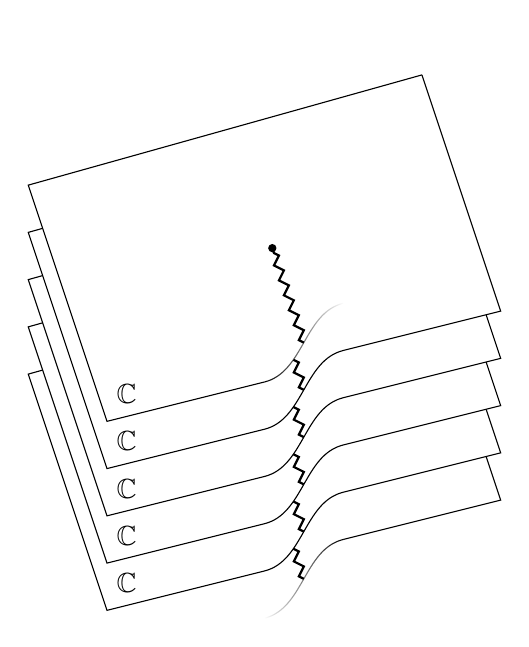
\begin{tikzpicture}
    \begin{scope}[shift={(0, -0.6)}]
      \draw [path fading=west] (2, 0.5) .. controls (2.5, 0.625) and (2.5, 1.375) .. (3, 1.5);
      \draw (3, 1.5) -- (5, 2) -- (4, 5);
      \draw [thick, decorate, decoration={zigzag, segment length=2mm, amplitude=0.5mm}] (2.5, 1) -- +(-0.4, 1.2);
    \end{scope}
    \foreach \x in {0, 1,2,3}{
      \begin{scope}[shift={(0, 0.6 * \x)}]
        \draw [fill=white] (4, 4.4) -- (-1, 3) -- (0, 0) -- (2, 0.5) .. controls (2.5, 0.625) and (2.5, 1.375) .. (3, 1.5) -- (5, 2) -- (4, 5);
        \draw [thick, decorate, decoration={zigzag, segment length=2mm, amplitude=0.5mm}] (2.5, 1) -- +(-0.4, 1.2);
        \node at (0, 0.1) [anchor = south west] {$\C$};
      \end{scope}
    }
    \begin{scope}[shift={(0, 2.4)}]
      \fill [white] (3.9, 4.4) -- (-1, 3) -- (0, 0) -- (2, 0.5) .. controls (2.5, 0.625) and (2.5, 1.375) .. (3, 1.5) -- (4.7, 2) -- (3.7, 5);
      \draw (4, 4.4) -- (-1, 3) -- (0, 0) -- (2, 0.5);
      \draw [path fading=east] (2, 0.5).. controls (2.5, 0.625) and (2.5, 1.375) .. (3, 1.5);
      \node at (0, 0.1) [anchor = south west] {$\C$};
      \draw [thick, decorate, decoration={zigzag, segment length=2mm, amplitude=0.5mm}] (2.5, 1) -- +(-0.4, 1.2) node [circ] {};
    \end{scope}
  \end{tikzpicture}
\end{center}
The idea is that traditionally, we are not allowed to cross branch cuts. Here, when we cross a branch cut, we will move to a different copy of $\C$, and this corresponds to a different branch of our function.

We will not say any more about this --- there is a whole Part II course devoted to these, uncreatively named IID Riemann Surfaces.

\subsubsection{Multiple branch cuts}
When there is more than one branch point, we may need more than one branch cut. For
\[
  f(z) = (z(z - 1))^{\frac{1}{3}},
\]
there are two branch points, at $0$ and $1$. So we need to branch cuts. A possibility is shown below. Then no curve can wrap around either $0$ or $1$.
\begin{center}
  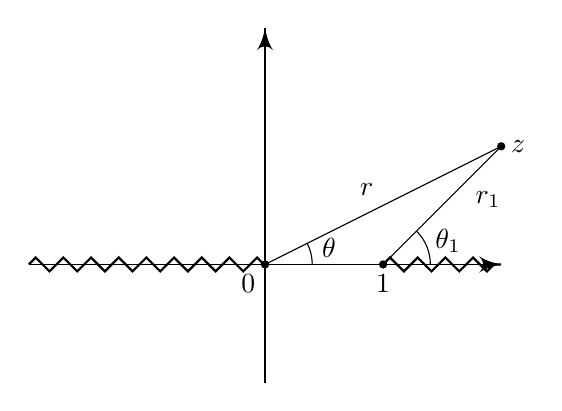
\begin{tikzpicture}[scale=1.5]
    \draw [->] (-2, 0) -- (2, 0);
    \draw [decorate, thick, decoration=zigzag] (-2, 0) -- (0, 0);
    \draw [decorate, thick, decoration=zigzag] (1, 0) -- (2, 0);
    \draw [->] (0, -1) -- (0, 2);
    \node [below] at (1, 0) {$1$};
    \node [anchor = north east] {$0$};
    \node [circ] at (1, 0) {};
    \node [circ] at (0, 0) {};

    \draw (0, 0) -- (2, 1) node [right] {$z$} node [circ] {} node [pos=0.5, anchor = south east] {$r$};
    \draw (1, 0) -- (2, 1) node [pos=0.7, anchor = north west] {$r_1$};

    \draw (0.4, 0) arc(0:26.565:0.4);
    \node at (0.4, 0.14) [right] {$\theta$};

    \draw (1.4, 0) arc (0:45:0.4);
    \node at (1.36, 0.2) [right] {$\theta_1$};
  \end{tikzpicture}
\end{center}
For any $z$, we write $z = re^{i\theta}$ and $z - 1 = r_1 e^{i\theta_1}$ with $\theta \in (-\pi , \pi]$ and $\theta_1 \in [0, 2\pi)$, and define
\[
  f(z) = \sqrt[3]{rr_1} e^{i(\theta + \theta_1)/3}.
\]
This is continuous so long as we don't cross either branch cut. This is all and simple.

However, sometimes, we need fewer branch cuts than we might think. Consider instead the function
\[
  f(z) = \log\left(\frac{z - 1}{z + 1}\right).
\]
Writing $z + 1 = r e^{i\theta}$ and $z - 1 = r_1 e^{i \theta_1}$, we can write this as
\begin{align*}
  f(z) &= \log (z - 1) - \log(z + 1)\\
  &= \log(r_1/r) + i(\theta_1 - \theta).
\end{align*}
This has branch points at $\pm 1$. We can, of course, pick our branch cut as above. However, notice that these two cuts also make it impossible for $z$ to ``wind around $\infty$'' (eg. moving around a circle of arbitrarily large radius). Yet $\infty$ is not a branch point, and we don't have to make this unnecessary restriction. Instead, we can use the following branch cut:
\begin{center}
  \begin{tikzpicture}[scale=1.5]
    \draw [->] (-2, 0) -- (2, 0);
    \draw [decorate, thick, decoration=zigzag] (-1, 0) -- (1, 0);
    \draw [->] (0, -1) -- (0, 2);
    \node [below] at (1, 0) {$1$};
    \node [below] at (-1, 0) {$-1$};
    \node [circ] at (1, 0) {};
    \node [circ] at (-1, 0) {};

    \draw (-1, 0) -- (2, 1) node [right] {$z$} node [circ] {} node [pos=0.5, anchor = south east] {$r$};
    \draw (1, 0) -- (2, 1) node [pos=0.7, anchor = north west] {$r_1$};

    \draw (-0.6, 0) arc(0:18.435:0.4);
    \node at (-0.8, 0.1) [above] {$\theta$};

    \draw (1.4, 0) arc (0:45:0.4);
    \node at (1.4, 0.2) [right] {$\theta_1$};
  \end{tikzpicture}
\end{center}
Drawing this branch cut is not hard. However, picking the values of $\theta, \theta_1$ is more tricky. What we really want to pick is $\theta, \theta_1 \in [0, 2\pi)$. This might not look intuitive at first, but we will shortly see why this is the right choice.

Suppose that we are unlawful and cross the branch cut. Then the value of $\theta$ passes through the branch cut, while the value of $\theta_1$ varies smoothly. So the value of $f(z)$ jumps. This is expected since we have a branch cut there. If we pass through the negative real axis on the left of the branch cut, then nothing happens, since $\theta = \theta_1 = \pi$ are not at a point of discontinuity.

The interesting part is when we pass through the positive real axis on the right of branch cut. When we do this, \emph{both} $\theta$ and $\theta_1$ jump by $2\pi$. However, this does not induce a discontinuity in $f(z)$, since $f(z)$ depends on the difference $\theta_1 - \theta$, which has not experienced a jump.

\subsection{M\"obius map}
The M\"obius map
\[
  z \mapsto w = \frac{az + b}{cz + d}
\]
with $ad - bc \not= 0$ is analytic except at $z = -\frac{d}{c}$. It is useful to consider it as a map from $\C^* \to \C^* = \C \cup \{\infty\}$, with
\[
  -\frac{d}{c} \mapsto \infty,\quad \infty \mapsto \frac{a}{c}.
\]
It is then a bijective map between $\C^*$ and itself, with the inverse being
\[
  w \mapsto \frac{-d w + b}{cw - a},
\]
another M\"obius map.

\begin{defi}[Circline]
  A \emph{circline} is either a circle or a line.
\end{defi}

The key property of M\"obius maps is the following:
\begin{prop}
  M\"obius maps take circlines to circlines.
\end{prop}
Note that if we start with a circle, we might get a circle or a line; if we start with a line, we might get a circle or a line.

\begin{proof}
  Any circline can be expressed as a circle of Apollonius,
  \[
    |z - z_1| = \lambda |z - z_2|,
  \]
  where $z_1, z_2 \in \C$ and $\lambda \in \R^+$.

  This was proved in the first example sheet of IA Vectors and Matrices. The case $\lambda = 1$ corresponds to a line, while $\lambda \not= 1$ corresponds to a circle. Substituting $z$ in terms of $w$, we get
  \[
    \left|\frac{-dw + b}{cw - a} - z_1\right| = \lambda \left|\frac{-dw + b}{cw - a} - z_2 \right|.
  \]
  Rearranging this gives
  \[
    |(cz_1 + d) w - (az_1 + b)| = \lambda|(cz_2 + d)w - (az_2 + b)|.\tag{$*$}
  \]
  A bit more rearranging gives
  \[
    \left|w - \frac{az_1 + b}{cz_1 + d}\right| = \lambda \left|\frac{cz_2 + d}{cz_1 + d}\right|\left|w - \frac{az_2 + b}{cz_2 + d}\right|.
  \]
  This is another circle of Apollonius.

  Note that the proof fails if either $cz_1 + d = 0$ or $cz_2 + d = 0$, but then $(*)$ trivially represents a circle.
\end{proof}

Geometrically, it is clear that choosing three distinct points in $\C^*$ uniquely specifies a circline (if one of the points is $\infty$, then we have specified the straight line through the other two points).

Also,
\begin{prop}
  Given six points $\alpha, \beta, \gamma, \alpha', \beta', \gamma' \in \C^*$, we can find a M\"obius map which sends $\alpha \mapsto \alpha', \beta \mapsto \beta'$ and $\gamma \to \gamma'$.
\end{prop}

\begin{proof}
  Define the M\"obius map
  \[
    f_1(z) = \frac{\beta - \gamma}{\beta - \alpha} \frac{z - \alpha}{z - \gamma}.
  \]
  By direct inspection, this sends $\alpha \to 0, \beta \to 1$ and $\gamma \to \infty$. Again, we let
  \[
    f_2(z) = \frac{\beta' - \gamma'}{\beta' - \alpha'} \frac{z - \alpha'}{z - \gamma'}.
  \]
  This clearly sends $\alpha' \to 0, \beta' \to 1$ and $\gamma' \to \infty$. Then $f_2^{-1} \circ f_1$ is the required mapping. It is a M\"obius map since M\"obius maps form a group.
\end{proof}

Therefore, we can therefore find a M\"obius map taking any given circline to any other.

\subsection{Conformal maps}
We've been doing quite a lot of stuff in this chapter. They are all going to magically come together in this section. But we first of all know what a conformal map is.

\begin{defi}[Conformal map]
  A \emph{conformal map} $f: U \to V$, where $U, V$ are \emph{open} subsets of $\C$, is one which is analytic with non-zero derivative.
\end{defi}
Although not part of the definition, it is usual (and helpful) to require that $f$ be one-to-one from $U$ to $V$.

Unfortunately, after many hundred years, we still haven't managed to agree on what being conformal means. An alternative definition is that a conformal map is one that preserves the angle (in both magnitude and orientation) between intersecting curves.

We shall show that our definition implies this is true; the converse is also true, but the proof is omitted. So the two definitions are equivalent.

\begin{prop}
  A conformal map preserves the angles between intersecting curves.
\end{prop}

\begin{proof}
  Suppose $z_1(t)$ is a curve in $\C$, parameterised by $t \in \R$, which passes through a point $z_0$ when $t = t_1$. Suppose that its tangent there, $z'_1(t_1)$, has a well-defined direction, ie. is non-zero, and the curve makes an angle $\phi = \arg z_1'(t_1)$ to the $x$-axis at $z_0$.

  Consider the image of the curve, $Z_1(t) = f(z_1(t))$. Its tangent direction at $t = t_1$ is
  \[
    Z_1'(t_1) = z_1'(t_1) f'(z_1(t_1)) = z_1'(t_0) f'(z_0),
  \]
  and therefore makes an angle with the $x$-axis of
  \[
    \arg (Z_1'(t_1)) = \arg(z_1'(t_1) f'(z_0)) = \phi + \arg f'(z_0),
  \]
  noting that $\arg f'(z_0)$ exists since $f$ is conformal, and hence $f'(z_0) \not= 0$.

  In other words, the tangent direction has been rotated by $\arg f'(z_0)$, and this is independent of the curve we started with.

  Now if $z_2(t)$ is another curve passing through $z_0$. Then its tangent direction will also be rotated by $\arg f'(z_0)$. The result then follows.
\end{proof}

Often, the easiest way to find the image set of a conformal map acting on a set $U$ is first to find the image of its boundary, $\partial U$, which will form the boundary $\partial V$ of $V$; but, since this does not reveal which side of $\partial V$ $V$ lies on, take a point of your choice within $U$, whose image will lie within $V$.

\begin{eg}\leavevmode
  \begin{enumerate}
    \item The map $z \mapsto az + b$, where $a, b \in \C$ and $a\not= 0$, is a conformal map. It rotates by $\arg a$, enlarges by $|a|$, and translates by $b$. This is conformal everywhere.
    \item The map $f(z) = z^2$ is a conformal map from
      \[
        U = \left\{z: 0 < |z| < 1, 0 < \arg z < \frac{\pi}{2}\right\}
      \]
      to
      \[
        V = \{w: 0 < |w| < 1, 0 < \arg w < \pi\}.
      \]
      \begin{center}
        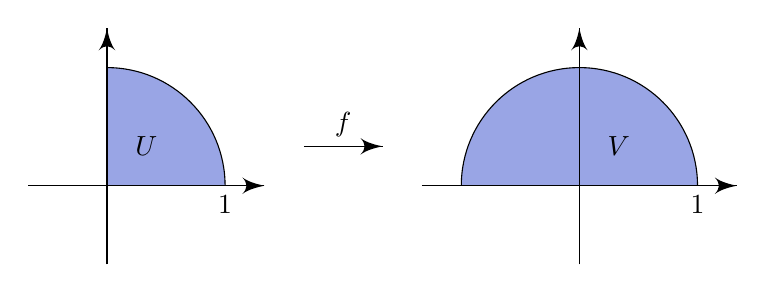
\begin{tikzpicture}
          \fill [mblue, opacity=0.5] (0, 0) -- (1.5, 0) arc(0:90:1.5) -- (0, 0);
          \draw [->] (-1, 0) -- (2, 0);
          \draw [->] (0, -1) -- (0, 2);
          \node [below] at (1.5, 0) {$1$};
          \draw (1.5, 0) arc(0:90:1.5);
          \node at (0.5, 0.5) {$U$};

          \draw [->] (2.5, 0.5) -- +(1, 0) node [pos=0.5, above] {$f$};
          \begin{scope}[shift={(6, 0)}];
            \fill [mblue, opacity=0.5] (0, 0) -- (1.5, 0) arc(0:180:1.5) -- (0, 0);
            \draw [->] (-2, 0) -- (2, 0);
            \draw [->] (0, -1) -- (0, 2);
            \node [below] at (1.5, 0) {$1$};
            \draw (1.5, 0) arc(0:180:1.5);
            \node at (0.5, 0.5) {$V$};
          \end{scope}
        \end{tikzpicture}
      \end{center}
      Note that the right angles between the boundary curves at $z = 1$ and $i$ are preserved, because $f$ is conformal there; but the right angle at $z = 0$ is not preserved because $f$ is not conformal there ($f'(0) = 0$). Fortunately, this does not matter, because $U$ is an \emph{open} set and does not contain $0$.
    \item How could we conformally map the left-hand half-plane
      \[
        U = \{z: \Re z < 0\}
      \]
      to a wedge
      \[
        V = \left\{w: -\frac{\pi}{4} < \arg w\leq \frac{\pi}{4}\right\}.
      \]
      \begin{center}
        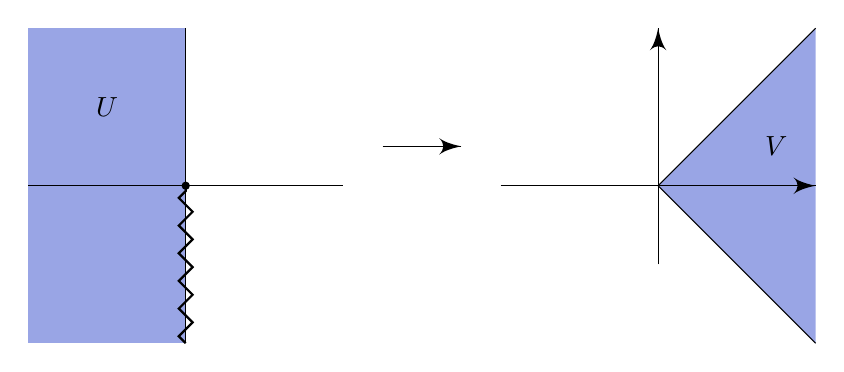
\begin{tikzpicture}
          \fill [mblue, opacity=0.5] (-2, 2) rectangle (0, -2);
          \draw (-2, 0) -- (2, 0);
          \draw (0, -2) -- (0, 2);
          \node at (-1, 1) {$U$};
          \node [circ] {};
          \draw [thick,decorate, decoration=zigzag] (0, -2) -- (0, 0);

          \draw [->] (2.5, 0.5) -- +(1, 0);
          \begin{scope}[shift={(6, 0)}];
            \fill [mblue, opacity=0.5] (2, 2) -- (0, 0) -- (2, -2);
            \draw [->] (-2, 0) -- (2, 0);
            \draw [->] (0, -1) -- (0, 2);
            \draw (2, 2) -- (0, 0) -- (2, -2);

            \node at (1.5, 0.5) {$V$};
          \end{scope}
        \end{tikzpicture}
      \end{center}
      We need to halve the angle. We saw that $z \mapsto z^2$ doubles then angle, so we might try $z^{\frac{1}{2}}$, for which we need to choose a branch. The branch cut must \emph{not} lie in $U$, since $z^{\frac{1}{2}}$ is not analytic on the branch cut. In particular, the principal branch does not work.

      So we choose a cut along the negative imaginary axis, and the function is defined by $r e^{i\theta} \mapsto \sqrt{r} e^{i\theta/2}$, where $\theta \in \left(-\frac{\pi}{2}, \frac{3\pi}{2}\right]$. This produces the wedge $\{z': \frac{\pi}{4} < \arg z' < \frac{3\pi}{4}\}$. This isn't exactly the wedge we want. So we need to rotate it through $-\frac{\pi}{2}$. So the final map is
      \[
        f(z) = -i z^{\frac{1}{2}}.
      \]
    \item $e^z$ takes rectangles conformally to sectors of annuli:
      \begin{center}
        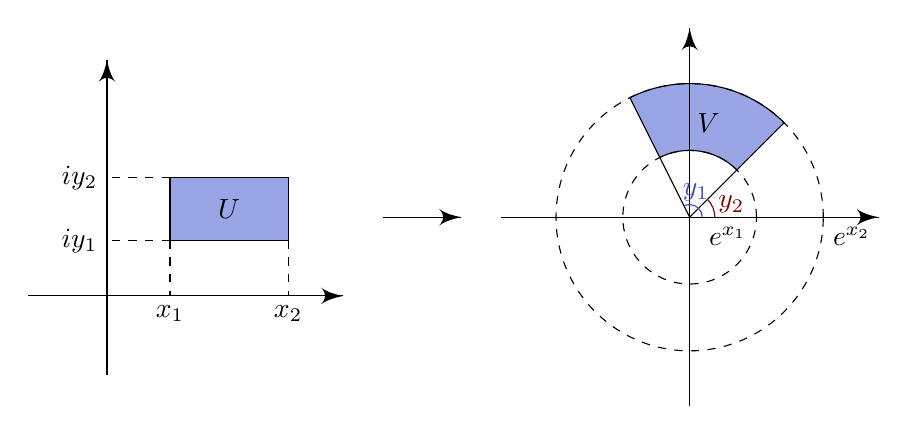
\begin{tikzpicture}
          \draw [->] (-1, 0) -- (3, 0);
          \draw [->] (0, -1) -- (0, 3);

          \draw [fill=mblue, fill opacity=0.5] (0.8, 0.7) rectangle (2.3, 1.5);
          \node at (1.55, 1.1) {$U$};
          \draw [dashed] (0.8, 0.7) -- (0, 0.7) node [left] {$iy_1$};
          \draw [dashed] (0.8, 1.5) -- (0, 1.5) node [left] {$iy_2$};
          \draw [dashed] (0.8, 0.7) -- (0.8, 0) node [below] {$x_1$};
          \draw [dashed] (2.3, 0.7) -- (2.3, 0) node [below] {$x_2$};

          \draw [->] (3.5, 1) -- +(1, 0);
          \begin{scope}[shift={(7.4,1)}, scale=0.8];
            \draw [fill=mblue, fill opacity=0.5] (0.75, 0.75) arc(45:116.565:1.0607) -- (-0.94868, 1.89737) arc(116.565:45:2.1213) -- cycle;

            \draw [->] (-3, 0) -- (3, 0);
            \draw [->] (0, -3) -- (0, 3);

            \draw (0, 0) -- (0.75, 0.75);
            \draw (0, 0) -- (-0.47434, 0.94868);
            \draw [dashed] circle [radius=2.1213];
            \draw [dashed] circle [radius=1.06066];

            \node [anchor = north east] at (1.0606, 0) {$e^{x_1}$};
            \node [anchor = north west] at (2.1213, 0) {$e^{x_2}$};

            \draw [mblue] (0.2, 0) arc(0:116.565:0.2);
            \node [mblue] at (0.1, 0.1) [above] {$y_1$};
            \draw [mred] (0.4, 0) arc(0:45:0.4);
            \node [mred] at (0.3, 0.2) [right] {$y_2$};

            \node at (0.3, 1.5) {$V$};
          \end{scope}
        \end{tikzpicture}
      \end{center}
      With an appropriate choice of branch, $\log z$ does the reverse.
    \item M\"obius maps (which are conformal equivalence except at the point that is sent to $\infty$) are very useful in taking circles, or parts of them to straight lines, or vice versa.

      Consider $f(z) = \frac{z - 1}{z + 1}$ acting on the unit disk $U = \{z: |z| < 1\}$. The boundary of $U$ is a circle. The three points $-1, i$ and $+1$ lie on this circle, and are mapped to $\infty$, $i$ and $0$ respectively.

      Since M\"obius maps take circlines to circlines, the image of $\partial U$ is the imaginary axis. Since $f(0) = -1$, we see that the image of $U$ is the left-hand half plane.
      \begin{center}
        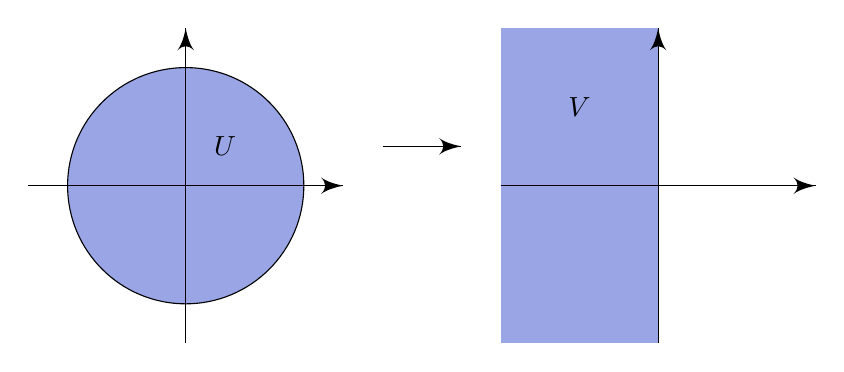
\begin{tikzpicture}
          \draw [fill=mblue, fill opacity=0.5] circle [radius=1.5];
          \draw [->] (-2, 0) -- (2, 0);
          \draw [->] (0, -2) -- (0, 2);
          \node at (0.5, 0.5) {$U$};

          \draw [->] (2.5, 0.5) -- +(1, 0);
          \begin{scope}[shift={(6, 0)}];
            \fill [mblue, opacity=0.5] (-2, 2) rectangle (0, -2);
            \draw [->] (-2, 0) -- (2, 0);
            \draw [->] (0, -2) -- (0, 2);
            \node at (-1, 1) {$V$};
          \end{scope}
        \end{tikzpicture}
      \end{center}
      We can derive this alternatively by noting
      \[
        w = \frac{z - 1}{z + 1} \Leftrightarrow z = -\frac{w + 1}{w - 1}.
      \]
      So
      \[
        |z| < 1 \Leftrightarrow |w + 1| < |w - 1|,
      \]
      ie. $w$ is closer to $-1$ than it is to $+1$, which describes precisely the left-hand half plane.

      In fact, this particular map $f(z) = \frac{z - 1}{z + 1}$ can be deployed more generally on quadrants, because it permutes $8$ divisions on the complex plane as follows:
      \begin{center}
        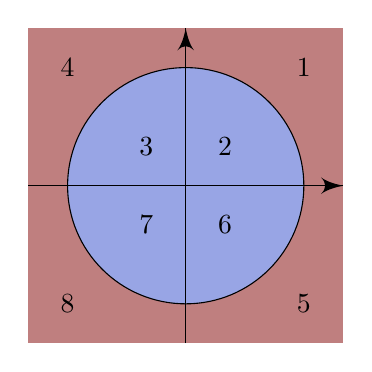
\begin{tikzpicture}
          \fill [mred, fill opacity=0.5] (-2, -2) rectangle (2, 2);
          \fill [white] circle [radius=1.5];
          \draw [fill=mblue, fill opacity=0.5] circle [radius=1.5];
          \draw [->] (-2, 0) -- (2, 0);
          \draw [->] (0, -2) -- (0, 2);
          \node at (0.5, 0.5) {$2$};
          \node at (-0.5, 0.5) {$3$};
          \node at (0.5, -0.5) {$6$};
          \node at (-0.5, -0.5) {$7$};

          \node at (1.5, 1.5) {$1$};
          \node at (-1.5, 1.5) {$4$};
          \node at (1.5, -1.5) {$5$};
          \node at (-1.5, -1.5) {$8$};
        \end{tikzpicture}
      \end{center}
      The map sends $1 \mapsto 2 \mapsto 3 \mapsto 4 \mapsto 1$ and $5 \mapsto 6 \mapsto 7 \mapsto 8 \mapsto 5$. In particular, this agrees with what we had above --- it sends the complete circle to the left hand half plane.
  \end{enumerate}
\end{eg}
\end{document}
